\documentclass[12pt]{article}
\usepackage[affil-it]{authblk}
\usepackage{verbatim}
\usepackage{graphicx}
\usepackage{float}
\usepackage[utf8]{inputenc}
\usepackage[top=2.5cm, bottom=2.5cm, left=2cm, right=2cm]{geometry}
\usepackage{graphicx}
\usepackage{color}
\usepackage{float}
\usepackage[small,bf]{caption}
\setlength{\captionmargin}{3pt}
\usepackage{multicol}
\usepackage{blindtext}
\usepackage{geometry}
\usepackage{subfigure}
\usepackage{enumerate}
\usepackage{scalefnt}

\title{Analysis of the STCP transport network}
\author{Diogo Bogas \\ 
        up201202482@fc.up.pt \\ 
        Departamento de Ciências de Computadores\\
        Faculdade de Ciências da Universidade do Porto\\
        }
\date{\today}


\begin{document}
\maketitle
%\newpage
\pagenumbering{arabic}


\section{Abstract}

This theme aims to do an initial analisys of the complex network that represents all the bus lines belonging to STCP. The student will start by creating the network, with automatic data extraction from sources like the website stcp.pt.
Then, with all the gathered data, there should be a preliminary data analisys with focus on node centrality, degree distribution and charateristic patterns.

\begin{multicols}{2}
\section{Introduction}

A network is a catalog of a system\textsc{\char13}s components often called nodes or vertexes and the direct interactions between them, called links or edges[1].
Some good examples of networks, are social networks like Facebook and Twitter.
This article uses networks to represent the services offered by a bus company operating in Porto, with the intent of answering some questions like : how many bus stops are there, which street has the most stops in it and what stops are the most "central". 
 

\section{Data Gathering and Processing}

\subsection{Data source}
The first decision made in this study wasn't what to study about the network, was to know were to get the data. 
The STCP website is a great place to start, as it has all the information on bus lines and bus stops. So, how do we get the information programatically?
The best way to do it, is to read the answer the server gives the client when a request is made. Luckily, this answer is in form of JSON objects, which are easily readable.
The information the site gives about bus stops and bus lines is enough for the common user, but we need more. There are some aspects we need to derive if we want to do a complete study on the proposed network. Therefore, every piece of information was locally stored.

\subsection{Data storing}
While reading the information from the server answers, i noticed that each time i wanted to read the data i had to , programatically,connect to the site ,and that took too long to be viable. 

A simple answer was to create two .txt files with the information gathered.

One of the files (AllLines.txt) has all the information about each bus line.
Each bus line is represented in a single line by a code, a direction, an integer that tells us the total number of stops in that line, and finally, all the stops that compose said line.

The other file (AllStops.txt) has all the information about all the stops.
Each stop is represented in a single line by a stop code, an address, a zone, a name and a pair of floating point numbers that represent it's geographical location. 

All of this information can be refreshed, as there are methods that do so.\\

There is the need for some structures in which to represent all this data we have, so it can be easily used to answer some of the questions raised above. The first type of information stored was information about lines, and the structure to represent a line is called BusLine:
\begin{itemize}
\item sentido
\item accessibility
\item code
\item description
\item pubcode
\item LineStops
\end{itemize}
Sentido is an integer that can take the values 0 or 1 and represents the direction a bus goes through a line. For example, the 207 line can go from Campanhã to Mercado da Foz, and from Mercado da Foz to Campanhã.\\
Accessibility is an integer that dictates the what special access conditions a bus line has. It can have wheel chair access, baby stroller access for example. Its a variable that was created when the information was being gathered, but ended up remaining in the structure.\\
Code is the server way to tell bus lines from each other.\\
Description is a String that tells us what appears in front of a bus that if going through a line.\\
PubCode is the people's way to tell lines from one another.\\
And lineStops is a List of Strings that represents the Stops that compose a line.\\

After knowing each line's composing stops, a list of all the stops was constructed, and the info for each stop was stored locally. The JAVA structure used is called Stop:
\begin{enumerate}
	\item stopCode, the ID of a Stop.
	\item address.
	\item zone, the part of the city a Stop belongs to.
	\item name, the way people know which stop is which.
	\item longitude.
	\item latitude.
	\item totalLinesServed, a number.
	\item linesServed, a list of the lines served.
	\item adjacentStops, the stops it can connect to.
	\item distanceBFS, an auxiliary variable to a BFS method.
\end{enumerate}

The last four variables are derived, and are used as auxiliary variables to some methods.\\
Thinking of this network as a graph, we already have the nodes in form of stops. Now we need to derive the edges. The edges are derived from the lines, taking into account the order each line goes through the stops it serves.The Edge structure used here is as follows:
\begin{enumerate}
	\item source;
	\item target;
	\item desc;
	\item weight;
\end{enumerate}

Source and Target define the edge, as the network is a directed graph. Desc is a String composed by both source and target stopcodes and the weight variable represents the number of lines that use that edge. 

To make this a more complete study, the stops were grouped by 2 characteristics, the first being their address. In this case, each street was a node, and an edge represents a trip between stops in two different streets. The node is represented by the BusStreet structure:
\begin{itemize}
	\item street
	\item stops, a list of all the stops in that street
	\item neighbours
	\item longitude;
	\item latitude;
\end{itemize}

The neighbours attribute was supposed to represent the streets adjacent to a particular street, but ended up not being used. The edges in this type of grouping are represented by AdressEdge:
	
\begin{itemize}
	\item src
	\item dest
	\item weight
	\item nome
\end{itemize}
	
The graph is directed still, weight is the number of lines that use that particular interaction and nome is a way to differentiate the edges, and is derived from the source and target streets.\\

The final type of grouping was by code prefix, which is easier to explain by an example:\\
In the AllStops.txt file there are two stops which stopcodes are TSL1 and TSL2. These were grouped in a single object that is named TSL. The structure to store this type of node is called Spot:

\begin{itemize}
	\item code
	\item stops
	\item LinesServed
\end{itemize}
	
Code is the way to tell Spots apart,stops is a list of stops the Spot has in itself and LinesServed is a list with all the lines that go through that Spot. The last variable is auxiliary to some method. The edges here are called SpotEdge:\\

\begin{itemize}
    \item from
    \item to
    \item weight
    \item name
\end{itemize}

"from" and "to" are the source and target Spots, weight and name, as the other types of edges are the number of lines that use the edge and a way to distinguish the edges respectively.\\
Some files, six to be more precise, were not included in this subsection, as they were generated with JAVA to be used by gephi.These files are described next subsection as the respective in the apendix, the generating methods come in the next subsection.

\subsection{Data processing and input creation}
	
	As mentioned before, Gephi was used to study the network. Gephi is a pretty powerful tool, but it requires some form of input. In this particular case .csv files. This subsection describes the methods that process the data (stored in any way described in the previous subsection) and generate the input Gephi needs.\\
	Still on the previous subsection, it was mentioned that there were 6 files left to describe. Three of these are groups of nodes, and the other three, groups of edges.\\
	
	
The first file to be described is called stops.csv , and it represents every single stop there is in this network. Five columns per stop :
	
	\begin{itemize}
		\item Id , is the code of each stop (the unique attribute).
		\item Address
		\item Zone
		\item name
		\item latitude
		\item longitude
	\end{itemize}
	
	To make this file, the method makeNodesCSV was created.
	It begins by printing "Id;Address;Zone;Name;Longitude;Latitude" in the first line of the output file. Then, for each stop it reads from the allStops.txt file, prints its attributes by the order sugested in the first line. As in the source file, each stop only takes one line.
	
	The second file to talk about is called allEdges.csv, with four columns per edge:
	
	\begin{itemize}
		\item Source stop
		\item Target stop
		\item type which is going to be directed for every edge in this study
		\item weight 
	\end{itemize}
	
	The generating method to this file is allEdgesCSV, and is similar to the nodes one.
	It also begins by printing what each column represents, (in this case "Source;Target;Type;Weight") and then for each edge it receives, prints its attributes in the order required. The source of the edges is an HashMap that comes from the getAllEdges method.\\

    Because the stops were also grouped by address, we need two more files for that, the node file for that grouping is called streetNodes, and the edges file is called streetEdges.\\
    The first is generated by the makeStreetNodeCSV method, which in the first line of the file writes "Id;TotalStops;Longitude;Latitude", and in each subsequent line writes each streetNode's values. \\
	The second file for this type of grouping  is generated by makeStreetEdgesCSV, and this file holds, for each edge, the weight, source, target and type.The weight in this particular case represents how many bus lines use that particular edge.\\
	%paragens por code aqui
	The last type of grouping is by code prefix. This allows us to group spots that are near each other (and potentially have a similar name ) in a single structure we call Spot:
\begin{itemize}
	\item code
	\item stops
	\item LinesServed
\end{itemize}
	
Code is the way to tell Spots apart,stops is a list of stops the Spot has in itself and LinesServed is a list with all the lines that go through that Spot.\\
The code variable derivation is easy to exemplify: in our list of Stops there are two whose codes are TSL1 and TSL2. These were grouped in a Spot which code is TSL.

The edges in this type of grouping are represented by the SpotEdge structure:
\begin{itemize}
\item from
\item to
\item weight
\item name
\end{itemize}

From and to are the source and target Spots, weight and name, as the other types of edges are the number of lines that use the edge and a way to distinguish the edges respectively.
	
\section{Results}
	This first image is the very first piece of information that our tool gave us, a visual representation of all 2416 stops in the network(not using any type of grouping), colored by zone.\\

\begin{figure}[H]
	\centering
	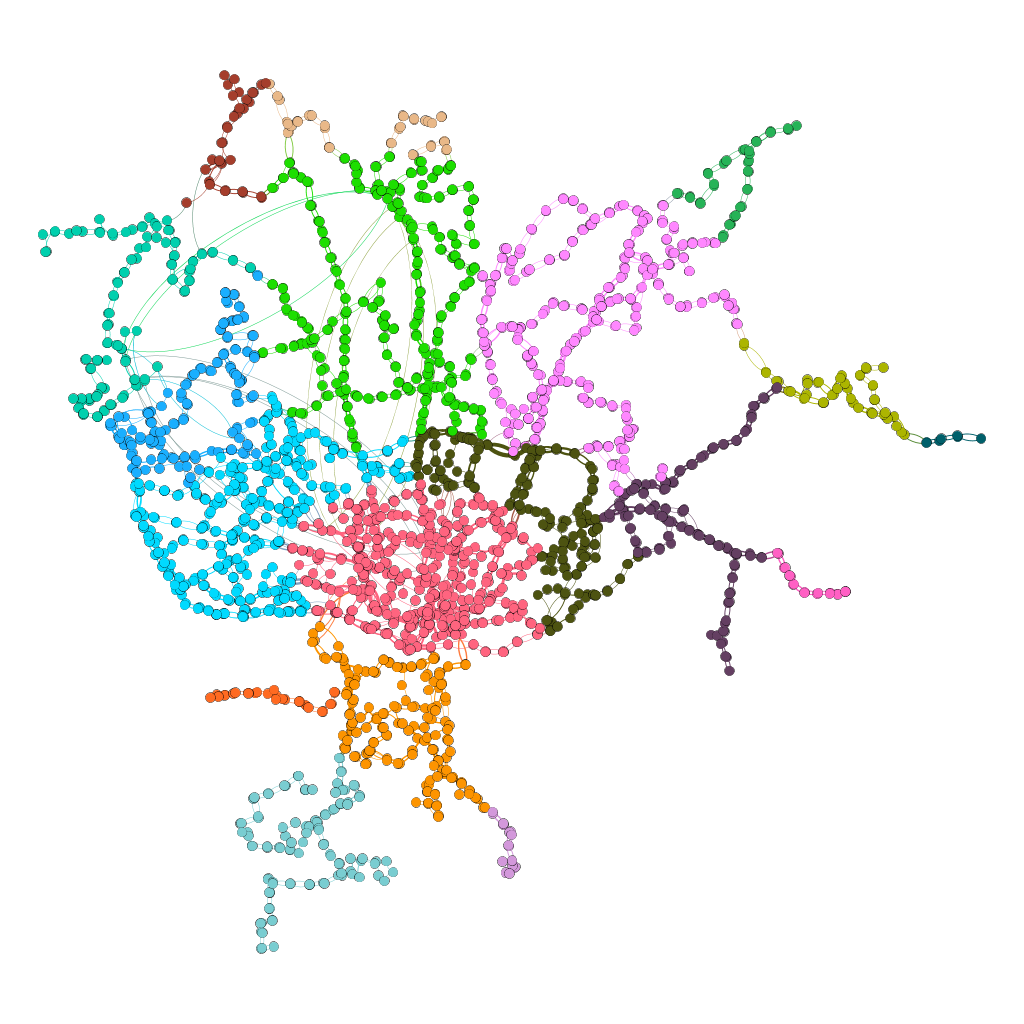
\includegraphics[scale=0.2]{simple_network}
	\caption{The network, without grouping, with stops colored by zones and shown according to geographical coordinates}
\end{figure}
The following image is the palette used to color the network shown above, and it ends up giving us how large is each zone relatively to it.\\
\begin{figure}[H]
	\centering
	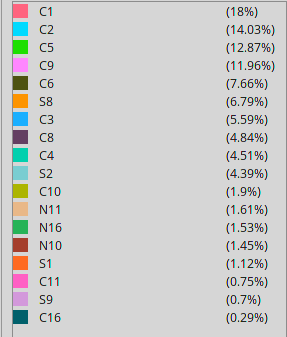
\includegraphics[scale=0.5]{legenda_simples}
	\caption{A table with all the zones, sorted according to size,displaying each zone's color}
\end{figure}

The second question raised in the Introduction section of this report was "Which Stop has the most lines going through it and how many times?". For this, it's better to group the stops by code, and answer a different question : "Which Spot has the most lines going through it?", as a Spot is much more influential than a simple Stop. Te answer to this, is in the table below,extracted from spotNodes.csv were the 5 most populated Spots are represented:
\begin{center}
\begin{tabular}[h]{ |c|c|c| }
\hline
    Id  & totalStops & linesServed\\
    TRD & 6          & 21 \\
    BCM & 5          & 20 \\
    BS  & 8          & 18 \\
    AAL & 6          & 17 \\
    CMO & 4          & 17 \\
\hline
\end{tabular}
\end{center}
Checking the Id's in the AllStops.txt file, we get, by ascending order:
Carmo,Aliados,Bom Sucesso,Casa da Música in Boavista and Trindade topping the list.Keep in mind that line 200 in direction 0 and 200 in direction 1 are two differetn lines.

In terms of streets, we want to know what is the street that holds the most stops. Checking the streetNodes.csv file and sorting by descending order the totalStops column, its verified that Estrada da circunvalação holds 86 stops. After some fact checking, it was verified that this street is 17 km long[2], which justifies a 64 stops difference to the 2nd street in this ranking. Follows the top 5:
\begin{center}
\begin{tabular}[h]{|l|ll|}
\hline
Street && Total Stops\\
ESTR.CIRCUNVALAÇÃO && 86\\
R.D.AFONSO HENRIQUES && 32\\
AV.BOAVISTA	&& 30\\
R.S.VICENTE	&& 23\\
R.COSTA CABRAL && 22\\
\hline
\end{tabular}
\end{center} 
Analising the nodes, with help from Gephi, we now look to the betweeness centrality. Betweeness measures how many times a given stop acts as a bridge in the shortest path between two other nodes. The next table shows, the "top 10" relative to betweeness:\\
\begin{tabular}[h]{|l|ll|}
\hline
	Nome 				&& Betweeness\\
	Trindade-C1 		&& 1145449.881\\%3840807\\	
	Graciosa-C1 		&& 771297.511\\%7531752\\		
	Bv.Cemitério-C1 	&& 754319.608\\%7318071\\			
	Moreira Sá-C1 		&& 736031.847\\%507471\\		
	Asprela-C6 			&& 678387.028\\%6322387\\	
	Av.Aliados-C1 		&& 644478.771\\%9011271\\
	Trindade-C1			&& 612273.626\\%8018036\\
	IPO(Circunval.)-C6 	&& 611095.614\\%6827459\\
	Areosa-C6 			&& 601167.850\\%6726616\\
	Casa da Música-C1 	&& 583327.933\\%8578992\\ 
\hline
\end{tabular}


There is a very noticeable pattern, most of the Stops shown above, belong to C1 zone, the center of the network.

\section{Conclusion}
	The results that we obtained colide with the reality.It was expected that the centre of Porto was the most busy zone of the entire network, and proof of that, is that C1 is the biggest zone,and most of it's Stops have the biggest Betweeness in the entire graph. The prior knowledge i had about the service this company provides, and the city itself, helped me as a "sanity check" as the data was processed. This study also allowed me to get a deeper understanding of Graph theory , and it's applications in real life situations.
\section{References}

[1] Albert-László Barabasi, Network Science\\[0pt]
[2] https://pt.wikipedia.org/wiki/EN12	

\end{multicols}	
\end{document}